\documentclass[10pt,a4paper]{article}
\usepackage[T1]{fontenc}
\usepackage[utf8]{inputenc}
\usepackage{lmodern,booktabs,graphicx,geometry,microtype,hyperref}
\geometry{margin=20mm}
\hypersetup{hidelinks}
\title{Coordinated Exploration of Scheduled Transit Service in Rome}
\author{Hamza Abdul Kader\\Sapienza University of Rome}
\date{Visual Analytics 2026--27 \quad Working paper, 16 November 2026}
\begin{document}
\maketitle
\begin{abstract}
This paper presents a visual analytics system for exploring the published supply of Rome public transit service at the stop level. Seven interactive views (a geographic map, a principal-component scatterplot, an hourly profile, three distribution charts and a ranked stop list) share one stop selection and are coordinated in both directions: any view can set the selection by brushing or clicking, and every view redraws to show it. Each selection recomputes a selected-versus-remaining median scheduled-departure comparison. A GTFS feed downloaded on 16 November 2026 schedules 8,252 active stops and 1,153,216 qualifying stop-time departures for the upcoming Wednesday 18 November 2026. These counts describe a published plan, not service observed on that future date. The system exposes central service concentration and profile differences while separating schedule evidence from claims about observed reliability, passenger demand or accessibility.
\end{abstract}

\section{Problem and users}
Transit planners and transport researchers may need to find stops that warrant closer route-level study. A citywide count can locate busy hubs but hides differences between stops; a map preserves location but does not expose combinations of service volume, route diversity and time profile. We designed an exploratory path that moves from a geographic region to a multivariate service profile and back. The domain questions are where scheduled service is concentrated, whether a selected group has a different typical departure count from the rest, and how its departures are distributed over a day.

\section{Related work and design framework}
Munzner's nested model separates domain questions, data and task abstraction, visual encodings and algorithms; the companion project documents record decisions at these levels~\cite{munzner}. Sacha et al. describe interactions that connect dimensionality reduction to other views, including selection and emphasis~\cite{sacha}. We use a fixed PCA projection linked to a geographic view and to five further views. The GTFS Schedule Reference defines the source tables and the meaning of a stop-time departure; it also distinguishes scheduled times from observed operation~\cite{gtfs}. Roma Servizi per la Mobilit\`a publishes the Rome feed and notes that its service information can vary in operation~\cite{rsm}.

Prommaharaj et al.'s PubtraVis uses Calgary GTFS data to show transit operation through mobility, speed, flow, density, headway and analysis modules, including side-by-side comparisons~\cite{pubtravis}. Our smaller system concentrates on the stop as a multivariate unit: a selection made in any of seven linked views directly triggers a selected-versus-remaining calculation. PubtraVis also involved transit professionals in evaluation, whereas our present user definition remains an explicit assumption to validate.

\section{Data and abstraction}
We downloaded the official static GTFS ZIP on 16 November 2026 and selected service IDs active on 18 November using \texttt{calendar\_dates.txt}. We joined active trips, routes, stop times and stops. One application row is one active \texttt{stop\_id}. We excluded records explicitly marked as no-pickup and stops with invalid or out-of-bounds coordinates. The resulting subset has 8,252 active stops from 8,325 valid-coordinate stops, 38,558 active trips, 403 active routes and 1,153,216 scheduled stop-time departures. A stop is not a station complex: nearby platforms may have distinct IDs. Times after 24:00 are folded to their clock hour in the hourly display but remain part of the chosen GTFS service day.

The five PCA inputs are log scheduled departures, log distinct routes, morning (07--09) departure share, evening (17--19) share and rail-mode share. The first two are counts; the last three are proportions. Each feature is clipped at its 1st and 99th percentiles for PCA only and then standardized. Raw counts remain in the numerical comparison. Singular-value decomposition yields the projection; signs are set so positive PC1 corresponds to more departures and positive PC2 to larger morning share. PC1 explains 36.62\% and PC2 28.09\% of feature variance.

\begin{figure}[t]
\centering
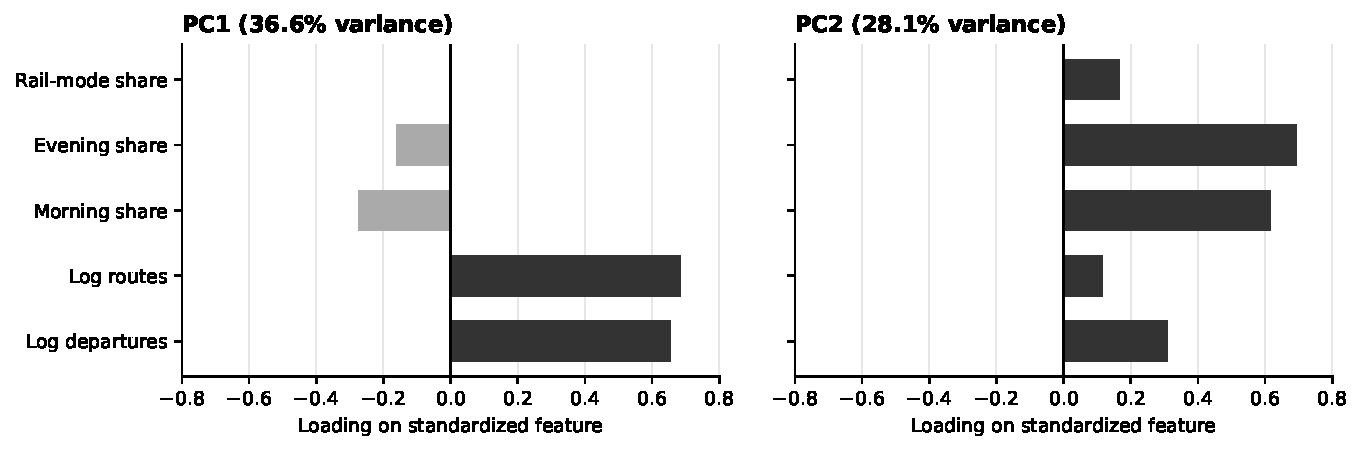
\includegraphics[width=.9\linewidth]{figures/pca_loadings.pdf}
\caption{Feature loadings for the two displayed principal components. Positive PC1 weights emphasize schedule volume and distinct routes; positive PC2 weights emphasize morning and evening shares. Signs were fixed for interpretability.}
\label{fig:loadings}
\end{figure}

\begin{table}[h]
\centering
\caption{Audit of the selected GTFS service date. Counts refer to published schedule records.}
\begin{tabular}{lr}
\toprule
Measure & Count \\
\midrule
Stops with bounded, valid coordinates & 8,325 \\
Active stops after date join & 8,252 \\
Active trips & 38,558 \\
Active routes & 403 \\
Eligible stop-time departures & 1,153,216 \\
\bottomrule
\end{tabular}
\label{tab:audit}
\end{table}

\section{Views and interaction}
The dashboard has seven views. All of them read and write one shared state: a set of stop indexes. A view \emph{sets} the selection when the analyst brushes or clicks it, and \emph{shows} the selection whenever any view changes it, so coordination runs in both directions for every pair of views (Table~\ref{tab:views}). A new interaction replaces the previous selection and the status line names the view and the range that produced it.

\begin{table}[h]
\centering
\caption{The seven coordinated views. Each sets the shared stop selection and redraws to show it.}
\label{tab:views}
\small
\begin{tabular}{p{.20\linewidth}p{.36\linewidth}p{.36\linewidth}}
\toprule
View & Sets the selection by & Shows the selection as \\
\midrule
01 Map & rectangle brush or stop click & dark stop marks \\
02 PCA & rectangle brush or stop click & dark stop marks \\
03 Hourly profile & dragging clock hours: stops whose busiest scheduled hour lies in the range & selection's share of departures per hour beside all stops \\
04 Departures & dragging logarithmic count bins & share of the selection's stops per bin beside all stops \\
05 Routes & dragging route-count bins & as view 04 \\
06 Distance & dragging distance bands from Termini & as view 04 \\
07 Ranked stops & clicking a named stop & the twelve busiest stops inside the selection \\
\bottomrule
\end{tabular}
\end{table}

The map places each stop by published longitude and latitude; the PCA scatterplot places the same stops by PC1 and PC2, allowing the analyst to find similar service profiles before locating them geographically. Views 03--06 are grouped bar charts in which a light bar gives the distribution for all stops and a dark bar the distribution for the selection, each as a share of its own group, so a small selection remains comparable with the city. View 03 plots shares of departures by clock hour; because it is brushed by hour, it selects stops by their busiest scheduled hour. View 07 ranks the busiest stops within the current selection, offering named entry points. The selection panel reports selected and remaining median scheduled departures per stop, their arithmetic difference, median distinct routes, rail-mode share and median distance from Termini. The calculation therefore follows a visual interaction rather than a menu filter.

\begin{figure}[!htbp]
\centering
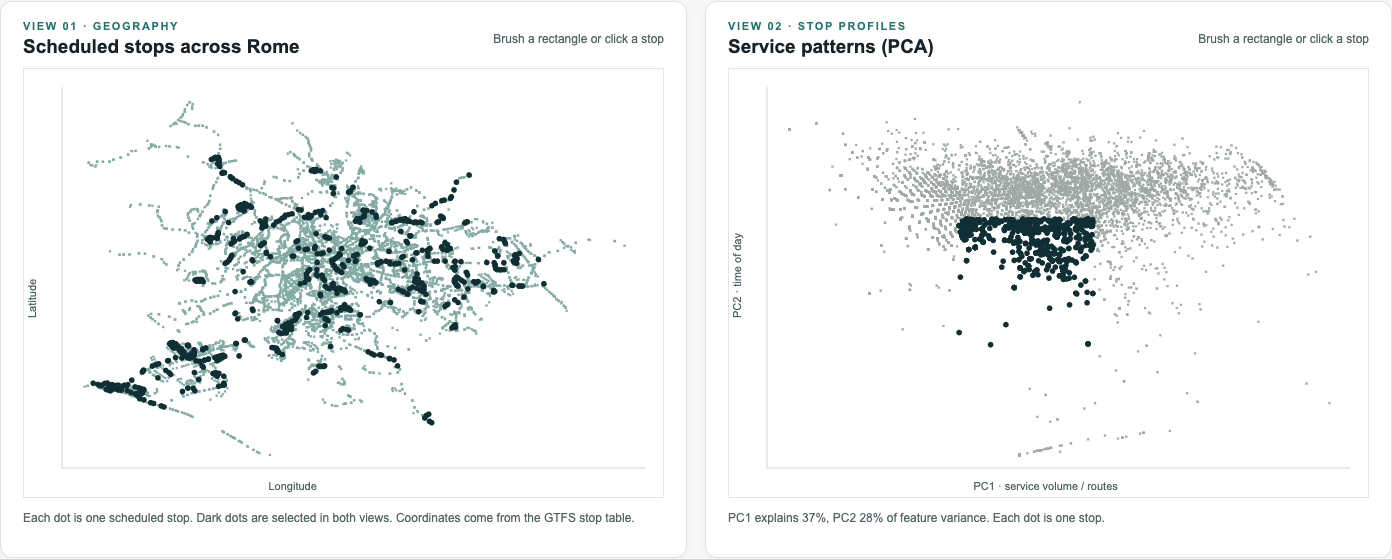
\includegraphics[width=.92\linewidth]{coordinated_views.png}\\[2pt]
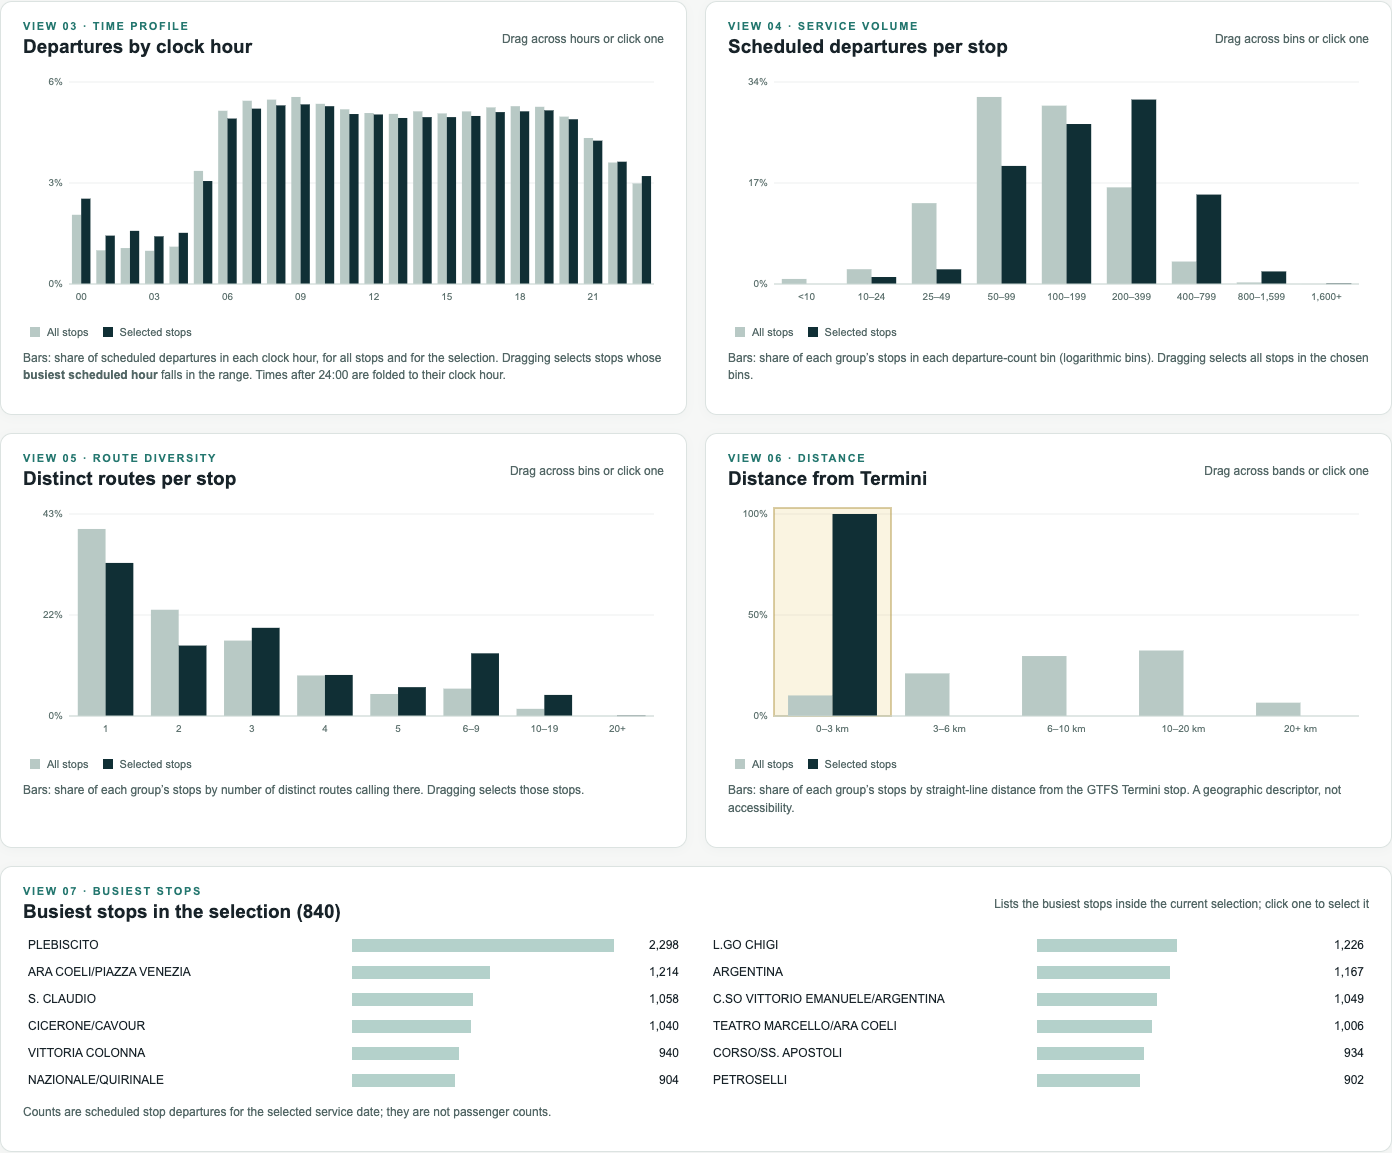
\includegraphics[width=.72\linewidth]{coordinated_detail.png}
\caption{A click on the 0--3\,km band in view 06 selects 840 stops. The map and PCA show them as dark marks; views 03--05 compare their distributions (dark) with all stops (light); view 07 (not shown) lists the busiest stops inside the selection. The PCA axes remain fixed across selections.}
\label{fig:views}
\end{figure}

The encoding uses geographic position for location and PCA position for multivariate profile. Selection is shown with dark marks or bars against muted marks in every view. Text labels and exact values accompany the visual density. We rejected a choropleth because aggregating into areas would hide adjacent stops with different schedules. We rejected recomputing PCA after every brush because moving axes would make before-and-after comparison unstable. In the bar views we rejected filtering unselected stops away, because the light all-stops distribution is the baseline the dark selection is read against. The two-dimensional projection leaves 35.29\% of standardized feature variance outside the display; proximity in the scatterplot is only a summary, not proof of equivalent service.

\section{Exploratory findings and validation}
In one usage scenario, the analyst clicks the 0--3\,km distance band. That visual action selects 840 stops, highlights their positions in the map and fixed PCA projection, and recomputes a median of 195.5 scheduled departures per selected stop versus 96 for the 7,412 remaining stops; median distinct routes are three versus two. The analyst can then brush a PCA region to locate a narrower service profile. This is a descriptive contrast for the dated schedule, not an effect of distance.

The feed's busiest stop ID in this analysis is PLEBISCITO, with 2,298 scheduled departures across 32 distinct routes. This is a count of published stop-time records, not passengers. Stops with PC1 greater than 1 (1,953 stops) have a median of 250 departures and five routes per stop; stops with PC1 below $-1$ (2,375 stops) have medians of 46 departures and one route. These are exploratory projection thresholds. Because departure count and route diversity are inputs to PC1, the separation confirms the component's interpretation and is not an independent discovery about service equity. For PC2 greater than 1, the morning/evening shares of all departures are 18.3\% and 17.7\%; below $-1$, they are 12.6\% and 11.6\%. This suggests a useful time-profile contrast to investigate further, while leaving route composition and geography as possible explanations.

As a separate descriptive check on the geographic pattern, we measured straight-line distance from the GTFS Termini stop coordinate (41.901308, 12.500433). Median scheduled departures per stop are 195.5 within 3 km (840 stops), 136 from 3--6 km (1,741), 124 from 6--10 km (2,450), 71 from 10--20 km (2,676), and 56 from 20--60 km (545). Figure~\ref{fig:radius} shows the distributions rather than only those medians, along with daily time profiles for the nearest and 10--20 km groups. The central group has a larger share of departures at 00--04 than the 10--20 km group; both have broad daytime service. Distance is a geographic descriptor, not a measure of accessibility or service quality.

\begin{figure}[!htbp]
\centering
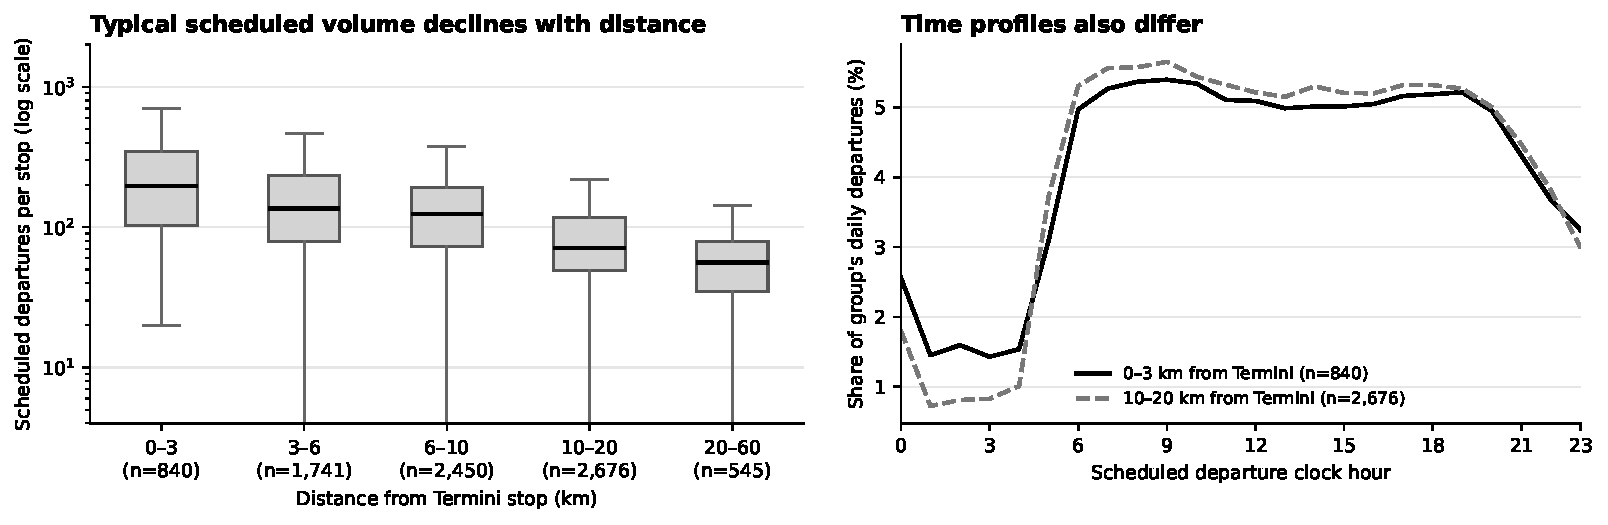
\includegraphics[width=\linewidth]{figures/service_radius.pdf}
\caption{Independent descriptive check of the dated GTFS snapshot. Left: scheduled departures per stop by straight-line distance from Termini, with boxes spanning the interquartile range and whiskers extending to 1.5 times that range; outliers are omitted for legibility. Right: each group's scheduled departures as a share of its own daily total by clock hour. The line styles remain distinguishable in grayscale.}
\label{fig:radius}
\end{figure}

A headless-browser test makes a selection from each of the seven views in turn and verifies that the selection count, status line and every other view change; it also checks a named-stop value against the prepared data, clearing and the absence of JavaScript errors. In one headless Chrome run the page loaded in 595\,ms and each of the seven selections, including simulated pointer input and the redraw of all views, completed in 51--194\,ms. A target-user walkthrough and repeated performance tests remain necessary before final submission. The one-day schedule says nothing about actual arrival times, cancellations, crowding, ridership or the population near a stop. The static feed can also change between publication dates.

\section{Discussion and threats to validity}
Bidirectional coordination across seven views supports different analytical starts. A geographic brush tests whether a place contains a mix of service profiles. A PCA brush tests whether a profile is spatially concentrated or scattered. A brush on the distance, route or departure distribution starts from a single attribute and reveals where those stops are and how they differ on the others; an hour brush asks where stops with an early or late peak lie. The comparison cards keep both the selected and remaining denominators visible. This matters because a large absolute number of departures may describe a few central stops, while a broad peripheral selection can contain many lower-volume stops. The hourly view gives an additional check: two groups with similar daily medians may serve different parts of the day.

The interpretation is sensitive to the unit of analysis. A physical interchange may contain multiple GTFS stop IDs, while a single stop ID can serve many routes. We therefore describe results as \emph{per-stop scheduled records}, not station capacity or network accessibility. The PCA features contain overlapping information: departures and route count are correlated, and morning and evening shares depend on the same total. Their loadings are descriptive rather than independent effects. The projection also compresses 35.29\% of standardized variance into unshown components. Comparing the selected medians with the full unselected group does not control for route type, geography or stop function, so a difference should lead to a more specific follow-up question, not a policy ranking.

The next validation step is to ask a target user to perform a geographic comparison and a profile-to-map lookup without guidance, then note where labels or encodings cause uncertainty. A future version could add spatial zoom, route-level details and an archived multi-date feed. Observed arrival records and passenger counts would be needed for reliability or demand questions.

\begin{thebibliography}{9}
\bibitem{munzner} T. Munzner, ``A nested model for visualization design and validation,'' \emph{IEEE TVCG}, 15(6), 2009. doi:10.1109/TVCG.2009.111.
\bibitem{sacha} D. Sacha et al., ``Visual interaction with dimensionality reduction: A structured literature analysis,'' \emph{IEEE TVCG}, 23(1), 2017. doi:10.1109/TVCG.2016.2598495.
\bibitem{gtfs} MobilityData, \emph{GTFS Schedule Reference}. \url{https://gtfs.org/documentation/schedule/reference/}.
\bibitem{rsm} Roma Servizi per la Mobilit\`a, \emph{Open data e controllo satellitare del trasporto pubblico (AVM)}. \url{https://romamobilita.it/sistemi-e-tecnologie/open-data/}. Accessed 16 November 2026.
\bibitem{pubtravis} P. Prommaharaj et al., ``Visualizing public transit system operation with GTFS data: A case study of Calgary, Canada,'' \emph{Heliyon}, 6(4), e03729, 2020. doi:10.1016/j.heliyon.2020.e03729.
\end{thebibliography}
\end{document}
